\subsection{Classifying Spectra}
\subsubsection{Simple Spectrum Classification}
After training the model was tested on a ``base case'', that is accumulated spectrum of copper PCB shown in \prettyref{fig:spectra-comparison}.
The output probabilities are visible on \prettyref{fig:copper-pcb-classification}.

\begin{figure}[H]
  \centering
  \includesvg[width=0.7\textwidth]{img/spectra-comparison.svg}
  \caption{Real and artificial spectrum comparison}
  \label{fig:spectra-comparison}
\end{figure}


\begin{figure}[H]
  \centering
  \includesvg[width=0.8\textwidth]{img/classification-results.svg}
  \caption{Classification results}
  \label{fig:copper-pcb-classification}
\end{figure}

For this simple case, the results are satisfactory.

\subsubsection{Classification Of Clustered Spectra}
Now, while having in mind that the model is far (\textbf{f a r}) from ideal, the results of clustered spectra classification can be presented. 
Spectra were clustered, accumulated and preprocessed as presented in \prettyref{sec:clustered-spectra}.
In the last step they were classified and probability maps for each element were visualized.
Due to probabilistic nature the maps they do not provide any quantitative information about elements.
Results are visible in \prettyref{fig:clusters-prob-sobieski}, \prettyref{fig:clusters-prob-gasecki} and \prettyref{fig:clusters-prob-matka-boska}.

\begin{figure}[H]
  \centering
  \includesvg[width=1\textwidth]{img/prediction_on_clusters_sobieski.svg}
  \caption{Probability maps of clustered spectra of ``Portrait of John III Sobieski in Karacena Scale Armour''}
  \label{fig:clusters-prob-sobieski}
\end{figure}

\begin{figure}[H]
  \centering
  \includesvg[width=1\textwidth]{img/prediction_on_clusters_gasecki.svg}
  \caption{Probability maps of clustered spectra of ``Portrait of Mieczysław Gąsecki''}
  \label{fig:clusters-prob-gasecki}
\end{figure}

\begin{figure}[H]
  \centering
  \includesvg[width=1\textwidth]{img/prediction_on_clusters_matka_boska.svg}
  \caption{Probability maps of clustered spectra of ``Mother of
God with the Child Eating an Apple''}
  \label{fig:clusters-prob-matka-boska}
\end{figure}

As expected, many false positives appeared in probability maps.
On the other hand results are not \emph{very} tragic. 
As one can see in \prettyref{fig:lach-comparison}, Pb was detected pretty well in places of higher concentration.
Little worse, but Fe was also registered.
Cu was mostly registered incorrectly because the escape photons of the $L_{\alpha}$ spectral line of Pb (7.59 keV) have energy close to the $K_{\alpha}$ line (8.05 keV) of Cu. 
This particular line was not included in the training process, so adding it could potentially improve the results.

\begin{figure}[htbp!]
  \centering
  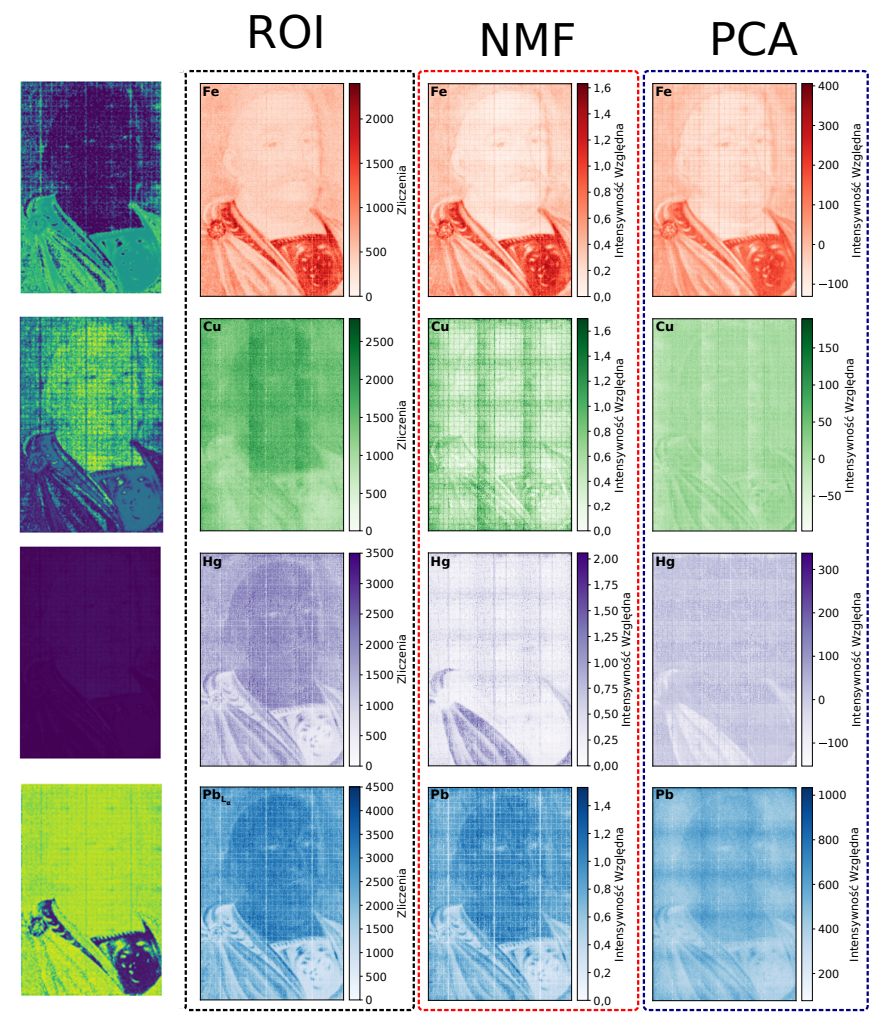
\includegraphics[width=1\textwidth]{img/comparison-lach.png}
  \caption{Comparison of probability maps with element distribution maps from \cite{Lach2022}}
  \label{fig:lach-comparison}
\end{figure}

\subsubsection{Classification Of Small Regions}
Another option was to classify single spectra or spectra averaged over small regions, e.g. $10\times10$ points. 

Savitzky–Golay filter implementation from \texttt{scipy} package was used to smooth spectra before further processing. Extrapolation step was omitted to reduce computational cost and issues with extrapolation of noisy spectra.
Example spectra are shown in \prettyref{fig:spectra}.

\begin{figure}[H]
    \begin{subfigure}{.5\linewidth}
        \centering
        \includesvg[width=1\textwidth]{img/spectrum_1x1.svg}
        \caption{Single spectrum }
        \label{fig:sub1}
    \end{subfigure}%
    \begin{subfigure}{.5\linewidth}
        \centering
        \includesvg[width=1\textwidth]{img/averaged_spectrum_processing_5x5.svg}
        \caption{Spectrum averaged over $5\times5$ region}
        \label{fig:sub2}
    \end{subfigure}\\[1ex]
    \centering
    \begin{subfigure}{0.5\linewidth}
        \centering
        \includesvg[width=1\textwidth]{img/averaged_spectrum_processing_10x10.svg}
        \caption{Spectrum averaged over $10\times10$ region}
        \label{fig:sub3}
    \end{subfigure}
    \caption{Example spectra}
    \label{fig:spectra}
\end{figure}

It is clearly visible that averaging over larger regions yield much clearer spectra, but it must be kept in mind that spatial resolution is lost in this way.

Resulting probability maps for different region sizes are shown in \prettyref{fig:10x10-point-sobieski}, \prettyref{fig:5x5-point-sobieski} and \prettyref{fig:single-point-sobieski}.

\begin{figure}[htbp!]
  \centering
  \includesvg[width=1\textwidth]{img/prediction_on_averaged_segments_10x10_sobieski.svg}
  \caption{Probability maps calculated over $10\times10$ segments of ``Portrait of John III Sobieski in Karacena Scale Armour''}
  \label{fig:10x10-point-sobieski}
\end{figure}

\begin{figure}[htbp!]
  \centering
  \includesvg[width=1\textwidth]{img/prediction_on_averaged_segments_5x5_sobieski.svg}
  \caption{Probability maps calculated over $5\times5$ segments of ``Portrait of John III Sobieski in Karacena Scale Armour''}
  \label{fig:5x5-point-sobieski}
\end{figure}

\newpage
\begin{figure}[H]
  \centering
  \includesvg[width=1\textwidth]{img/prediction_on_single_spectra.svg}
  \caption{Probability maps calculated over single points of ``Portrait of John III Sobieski in Karacena Scale Armour''}
  \label{fig:single-point-sobieski}
\end{figure}
It seems that despite the author's concerns classifying single works quite good.
As \prettyref{fig:single-point-sobieski} shows, it is the only case when the model succeeded to somehow register Hg element, which was invisible in \prettyref{fig:lach-comparison}.
However, it took a lot of time. 
Inference of all spectra took approximately 20 minutes on T4 GPU for this fairly small model ($10^6$ parameters).

Similar probability maps of another two paintings are visible on \prettyref{fig:single-point-gasecki} and \prettyref{fig:single-point-matka-boska}.

\begin{figure}[htbp!]
  \centering
  \includesvg[width=1\textwidth]{img/prediction_on_single_spectrum_gasecki.svg}
  \caption{Probability maps calculated over single points of ``Portrait of Mieczysław Gąsecki''}
  \label{fig:single-point-gasecki}
\end{figure}

\begin{figure}[htbp!]
  \centering
  \includesvg[width=1\textwidth]{img/prediction_on_single_spectrum_matka_boska.svg}
  \caption{Probability maps calculated over single points of ``Mother of
God with the Child Eating an Apple''}
  \label{fig:single-point-matka-boska}
\end{figure}